\section{Authorization Components}

The authorization components are those which are responsible for managing access
control for \solt{contract}[s]. This section builds varying complexities of
access control beginning with:

\begin{enumerate}
  \item \emph{Primitive Contract Ownership}, which reviews basic access control
    mechanisms; then

  \item \emph{Generalized Access Control}, which introduces components for
    guarding access to resources; next

  \item \emph{Access Control Lists}, which demonstrate components for
    constructing and managing access control lists and integrating them with the
    components introduced for generalized access control; and finally,

  \item \emph{Registries}, which demonstrates voter registry components
    leveraging the aforementioned components to build and manage voter
    databases.
\end{enumerate}

\begin{figure}[H]
  \centering
  \figurepdf[width=\textwidth]{authorization}
  % 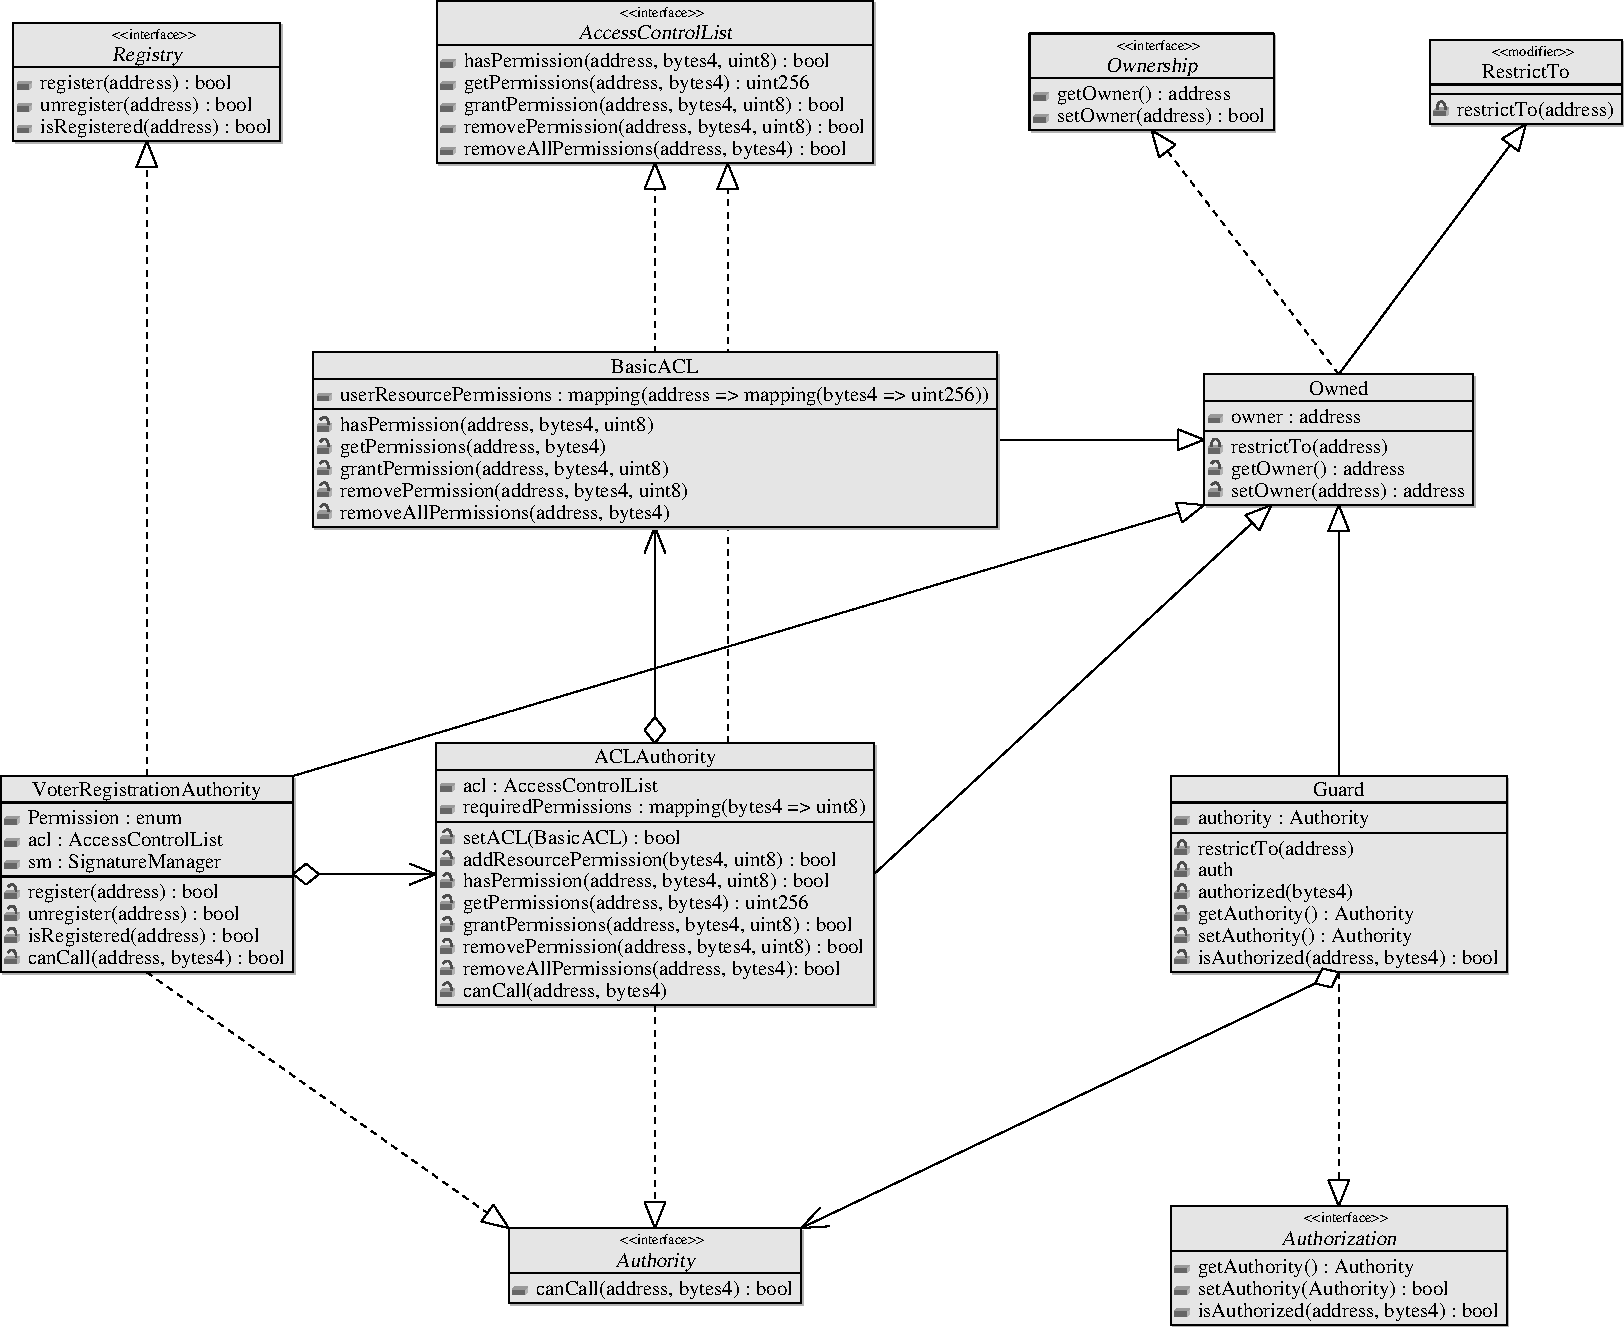
\includegraphics[width=\textwidth]{figures/authorization/figure}
  % \includestandalone[width=\textwidth]{\fig{authorization}}
  \caption{Authorization dependency graph modeling.}% \label{fig:authorization}
\end{figure}

% Sub-section: Managing Contract Ownership
\subsection{Primitive Contract Ownership}

Managing \solt{contract} ownership is one of the most basic forms of access
control in the Ethereum ecosystem. Here we introduce:

\begin{enumerate}
  \item \sol{interface Ownership}, which defines \solt{function}[s] to
    express \solt{contract} ownership,
  \item \sol{contract RestrictTo}, which defines a \solt{modifier} for
    restricting access to \solt{function} calls based on an \solt{address}, and
  \item \sol{contract Owned}, a convenience \solt{contract}, which provides an
    implementation of \sol{interface Ownership} and leverages
    \sol{contract RestrictTo}.
\end{enumerate}

\begin{figure}[H]
  \centering
  \figurepdf[]{ownership}
  \caption{Contract ownership dependency graph modeling.}\label{fig:ownership}
\end{figure}

\subsubsection{Contract RestrictTo}

The \solt{contract}, \sol{contract RestrictTo}, introduces a single
\solt{modifier}, \sol{modifier restrictTo}, which requires the caller of the
\solt{function}, \sol{msg.sender}, to have the same \solt{address} as the
argument, \sol{address _subject}, provided to the \solt{modifier} when called.

\begin{solidity}[contract RestrictTo]
contract RestrictTo {
  modifier restrictTo (address _subject) {
    require(msg.sender == _subject);
    _;
  }
}
\end{solidity}

\begin{code}
  \begin{modifiers}
    \item \sol{modifier restrictTo (address _subject)}, restricts access to
      \solt{function} calls based on an \solt{address} provided.

      \begin{displayquote}
        Restriction to \solt{function}[s] is accomplished by comparing the
        \solt{address} of the \solt{function} \emph{caller}, \sol{msg.sender},
        against the configured \solt{address}, \sol{address _subject}. If the
        \solt{address} of the \solt{msg.sender} does not match the
        \solt{address} of the \solt{_subject} then the \solt{require} statement
        will force the immediately arrest of \solt{contract} evaluation,
        \solt{revert} the \emph{state} of the \solt{contract}, refund any
        remaining \solt{gas}, \solt{gasleft()}, to the \emph{caller}, and
        exit.\footnotemark{}

        \todo{Should notes be documented differently?}
      \end{displayquote}

      \footnotetext{
        Note that the \emph{caller}, \sol{msg.sender}, of the \solt{function}
        will not necessarily be an \emph{external account}, e.g., human user;
        the \emph{caller} of the \solt{contract} \solt{function} may itself also
        be a \solt{contract}, i.e., a \emph{contract account}, which is calling
        the \solt{contract} \solt{function} from its own \solt{contract}
        \solt{function}.
      }

      \begin{parameters}
      \item \sol{address _subject}, the \emph{subject} who is to be granted
        access to the \solt{function}.

        \begin{displayquote}
          The \solt{address} of the \emph{subject} may be \emph{any} Ethereum
          account, including \emph{contract accounts}.
        \end{displayquote}
      \end{parameters}
  \end{modifiers}
\end{code}


\paragraph{Interface Ownership}

The \solt{interface}, \sol{interface Ownership}, introduces two
\solt{function}[s] for managing contract ownership:

\begin{enumerate}
  \item \sol{function getOwner}, which is expected to return the \solt{address}
        of the owner of the \solt{contract}, and
  \item \sol{function setOwner}, which is expected to update the \solt{address}
        of the owner of the \solt{contract}.
\end{enumerate}

\begin{solidity}[interface Ownership]
interface Ownership {
  function getOwner () public view returns (address _owner);
  function setOwner (address _owner) public returns (bool _success);
}
\end{solidity}

\begin{interface}
  \begin{functions}
    \item \sol{function getOwner ()}, returns the \solt{address} of the owner of
      the \solt{contract}.

      \begin{returns}
        \item \sol{address _owner}, the \emph{subject} representing the owner of
          the \solt{contract}.
      \end{returns}

    \item \sol{function setOwner (address _owner)}, updates the \solt{address}
      representing the owner of the \solt{contract}.

      % which accepts an \solt{address},
      % \sol{address _owner}, and is expected to update the owner of the
      % \solt{contract} and \solt{return} a \solt{bool}, \sol{bool _success},
      % which resolves to \solt{true} if the operation was successful; otherwise
      % \solt{false}.


      \begin{parameters}
      \item \sol{address _owner}, the \emph{subject} which is to be granted
        ownership of the \solt{contract}.\footnotemark{}

        \footnotetext{\label{param:address-owner}
          The \solt{address} of the \emph{subject} may be \emph{any} Ethereum
          account, including \emph{contract accounts}.
        }
      \end{parameters}

      \begin{returns}
      \item \sol{bool _success}, resolves to \solt{true} if the operation was
        successful; otherwise \solt{false}.
      \end{returns}
  \end{functions}
\end{interface}


\subsubsection{Contract Owned}

A convenience \solt{contract}, \sol{contract Owned}, implements
\sol{interface Ownership} and extends \sol{contract RestrictTo}; in doing so,
\sol{contract Owned} provides a simple mechanism for expressing \solt{contract}
ownership, extending \sol{contract Owned}; e.g., \sol{contract MyContract is
Owned {}}.

% Upon creation, the \solt{constructor} of this \solt{contract} sets the
% \solt{owner} property of the \solt{contract} to the \solt{address} which
% created the contract, and restricts future calls to the \sol{function
% setOwner} to the owner of the \solt{contract} by using the \sol{modifier
% restrictTo(owner)}.

\begin{solidity}[contract Owned]
contract Owned is RestrictTo, Ownership {
  address public owner;

  constructor () {
    owner = msg.sender;
  }

  function getOwner () public view returns (address _owner) {
    return owner;
  }

  function setOwner (address _owner) public restrictTo(owner) returns (bool _success) {
    owner = _owner;
    return true;
  }
}
\end{solidity}

\begin{state}
  \begin{public}
    \item \sol{address owner}, maintains the \solt{address} of the current
      \solt{owner} of the \solt{contract}.
  \end{public}
\end{state}

\begin{code}
  \begin{constructor}
    \item \sol{constructor ()}, upon creation and initialization of this
      \solt{contract} the \solt{constructor} sets the \sol{address owner}
      property of the \solt{contract} to the \solt{address} of the
      \solt{contract} creator, \sol{msg.sender}, i.e., the \emph{subject}
      submitting the \solt{CREATE} opcode.
  \end{constructor}

  \begin{functions}
    \item \sol{function getOwner ()}, returns the \solt{address} of the owner of
      the \solt{contract}.

      \begin{returns}
        \item \sol{address _owner}, the \emph{subject} representing the owner of
          the \solt{contract}.
      \end{returns}

    \item \sol{function setOwner (address _owner)}, updates the \solt{address}
      representing the owner of the \solt{contract}, effectively transferring
      ownership of the \solt{contract}.

      \begin{modifiers}
        \item \sol{modifier restrictTo (owner)}, restricts access to the
          \solt{function} such that \emph{only} the current \solt{owner} of the
          \solt{contract} can update/transfer ownership of the \solt{contract}.
      \end{modifiers}

      \begin{parameters}
        \item \sol{address _owner}, the \emph{subject} who is to be granted access
          to the \solt{function}.
      \end{parameters}

      \begin{returns}
        \item \sol{bool _success}, the \emph{subject} representing the owner of
          the \solt{contract}
      \end{returns}
  \end{functions}
\end{code}



% Sub-section: Generalizing Contract Access Control
\subsection{Generalizing Contract Access Control}

In order to generalize \solt{contract} access control we introduce:

\begin{enumerate}
  \item \sol{interface Authority}, which defines \solt{function}[s] to determine
    whether some \emph{subject} is permitted to access some \emph{resource},
  \item \sol{contract Authorization}, which defines a \solt{modifier} for
    restricting access to \solt{function} calls based on an \solt{address}, and
  \item \sol{contract Guard}, a convenience \solt{contract}, which provides an
    implementation of \sol{interface Authorization} by aggregating
    implementations of \sol{interface Authority}.
\end{enumerate}

Together these components allow us to provide a generalized access control
model; isolating and deferring the responsibilities of
authorization.% \footnotemark{}
\todo{Alternative names: Guard, Authority, Enforcer, Authorization}

% \footnotetext{
%   I think I would maybe prefer \sol{interface Authorization} to define
%   \sol{isAuthorized} and for \sol{interface Authority} to define
%   \sol{getAuthority} and \sol{setAuthority}.
%
%   A better name in that case might be \sol{interface AuthorityManager}.
% }

\begin{figure}[H]
  \centering
  \figurepdf[]{guard}
  \caption{Generalized contract access control.}% \label{fig:authorization}
  % 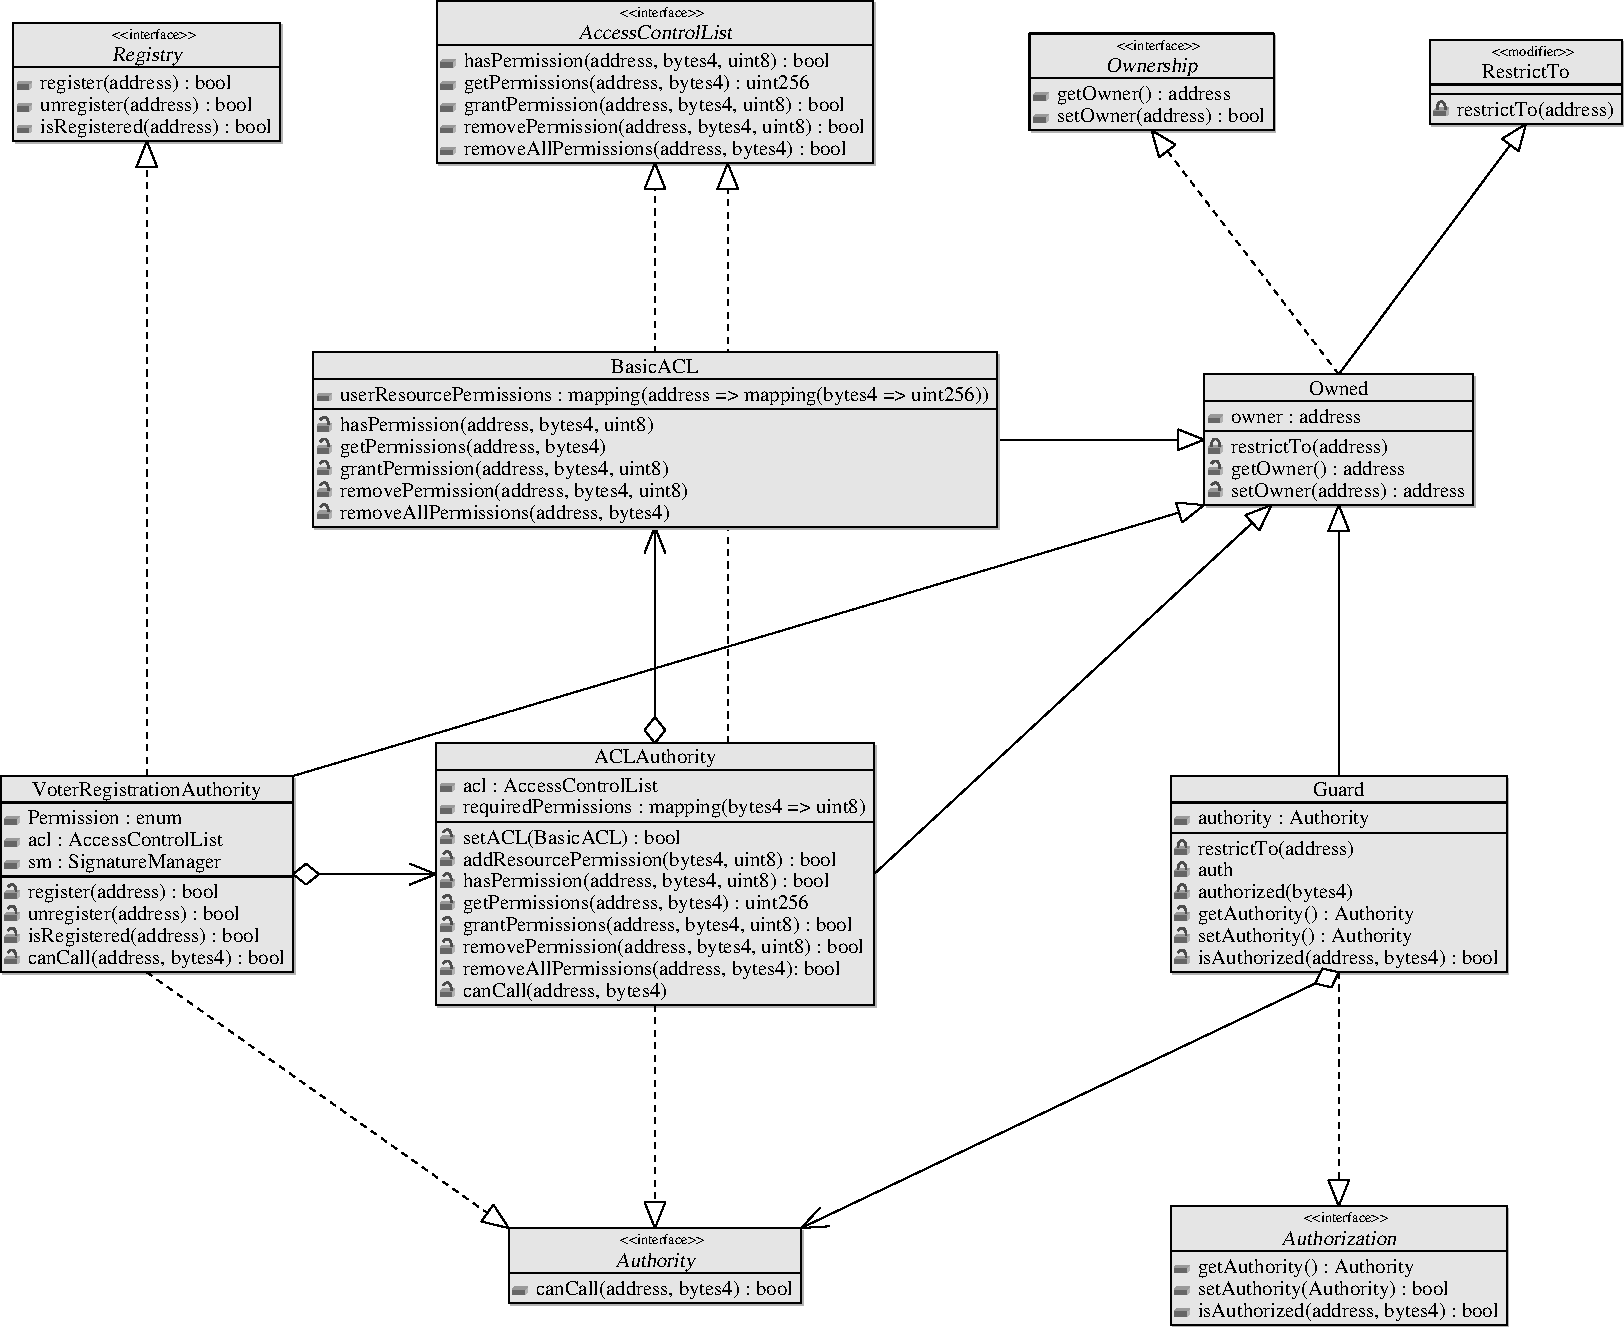
\includegraphics[width=\textwidth]{figures/authorization/figure}
  % \includestandalone[width=\textwidth]{\fig{authorization}}
\end{figure}

\subsubsection{Interface Authority}

The \solt{interface}, \sol{interface Authority}, introduces functionality for
managing whether some \emph{subject}, typically an Ethereum account represented
by \solt{address}, can access some \emph{resource}, typically an Ethereum
\solt{function} represented by \solt{function} signature, \solt{bytes4}. By
defining the \emph{resource} by it's \solt{function} signature and not by a
specific \solt{function} owned by a specific \solt{contract} we leave open the
possibility for managing \solt{contract} access control across
\solt{contract}[s], a functionality which will be necessary to build
pseudo-centralized registration authorities.

\begin{solidity}[interface Authority]
interface Authority {
  function canCall (address _subject, bytes4 _resource) public constant returns (bool _canCall);
}
\end{solidity}

\begin{interface}
  \begin{functions}
    \item \sol{function canCall (address _subject, bytes4 _resource)}, evaluates
      whether some \emph{resource}, \solt{contract function}, can be used by
      some \emph{subject}, Ethereum account.

      \begin{parameters}
        \item \sol{address _subject}, the \emph{subject}, Ethereum account,
          whose permissions are being evaluated.\footnotemark{}

          \footnotetext{
            The \solt{address} of the \emph{subject} may be \emph{any} Ethereum
            account, including \emph{contract accounts}.
          }

        \item \sol{bytes4 _resource}, the \emph{resource}, \solt{contract
          function}, which the \emph{subject's} permissions are being evaluated
          against.
      \end{parameters}

      \begin{returns}
        \item \sol{bool _canCall}, resolves to \solt{true} if the
          \emph{subject}, \sol{address _subject}, is permitted to access the
          \emph{resource}, \sol{bytes4 _resource}, otherwise \solt{false}.
      \end{returns}
  \end{functions}
\end{interface}


\subsubsection{Interface Authorization}

The \solt{interface}, \sol{interface Authorization}, introduces functionality
for managing authorities, \sol{function getAuthority()} and \sol{function
setAuthority()}, and also functionality similar to that of an \solt{Authority},
\sol{function isAuthorized()}.% \footnotemark{}

% \footnotetext{
%   If I don't update this to just be \sol{interface AuthorityManager} then I
%   should \emph{really} update \sol{interface Authority} to supply
%   \sol{function isAuthorized ()}, instead of \sol{function canCall()}, and
%   update this \solt{interface} to implement/extend \sol{interface Authority}.
% }

\begin{solidity}[interface Authorization]
interface Authorization {
  function getAuthority () public constant returns (address _authority);
  function setAuthority (address _authority) public returns (bool _success);
  function isAuthorized (address _subject, bytes4 _resource) public returns (bool _isAuthorized);
}
\end{solidity}

\begin{interface}
  \begin{functions}
    \item \sol{function getAuthority ()}, returns the \solt{address} of a
      \solt{contract} which implements the \solt{interface Authority}.

      \begin{returns}
        \item \sol{address _authority}, the \solt{address} of a \solt{contract}
          which implments the \solt{interface Authority}.
      \end{returns}

    \item \sol{function setAuthority (address _authority)}, updates the state of
      the \solt{contract} to to reflect the new \solt{contract} which provides
      an implementation of the \solt{Authority interface}.
      \todo{
        Make sure the Guard checks that the contract actually implements the
        interface!!!
      }

      \begin{parameters}
        \item \sol{address _authority}, the \solt{address} of a \solt{contract}
          which implements the \solt{interface Authority}.
      \end{parameters}

      \begin{returns}
        \item \sol{bool _success}, resolves to \solt{true} if the operation was
          successful; otherwise \solt{false}.
      \end{returns}

    \item \sol{function isAuthorized (address _subject, bytes4 _resource)},
      evaluates whether some \emph{subject}, Ethereum account, is authorized to
      access some \emph{resource}, \solt{contract function}.

      \begin{parameters}
        \item \sol{address _subject}, the \emph{subject}, Ethereum account,
          whose permissions are being evaluated.\footnotemark{}

          \footnotetext{
            The \solt{address} of the \emph{subject} may be \emph{any} Ethereum
            account, including \emph{contract accounts}.
          }

        \item \sol{bytes4 _resource}, the \emph{resource}, \solt{contract
          function}, which the \emph{subject's} permissions are being evaluated
          against.
      \end{parameters}

      \begin{returns}
        \item \sol{bool _isAuthorized}, resolves to \solt{true} if the
          \emph{subject}, \sol{address _subject}, is permitted to access the
          \emph{resource}, \sol{bytes4 _resource}, otherwise \solt{false}.
      \end{returns}
  \end{functions}
\end{interface}


\subsubsection{Contract Guarded}

The \solt{contract}, \sol{contract Guarded}, is a \solt{contract} which offers a
convenient mechanism for easily integrating generalized \solt{contract} access
control functionality; e.g., \sol{contract MyContract is Guarded {}}.
\solt{contract Guarded}, by virtue of implementing the \solt{Authorization
interface}, supports deferring access control responsibilities to an external
\solt{contract} which implements the \solt{Authority interface} while leaving
open the possibility for a \solt{contract} to provide its own access control
implementation by itself implementing the \solt{Authority interface}.

\todo{If I'm changing this from Guard to Guarded then I need to update all of
the references to Guard.}

\begin{solidity}[contract Guarded]
contract Guarded is Owned, Authorization {
  Authority public authority;

  function getAuthority () public constant returns (address _authority) {
    return address(authority);
  }

  function setAuthority (address _authority) public auth returns (bool _success) {
    authority = Authority(_authority);
    return true;
  }

  function isAuthorized (address _subject, bytes4 _resource) public returns (bool _isAuthorized) {
    if (_subject == address(this)) return true;
    if (authority == Authority(0)) return false;
    if (_subject == owner) return true;
    return authority.canCall(_subject, _resource);
  }

  modifier auth {
    assert(isAuthorized(msg.sender, msg.sig));
    _;
  }

  modifier authorized (bytes4 _resource) {
    assert(isAuthorized(msg.sender, _resource));
    _;
  }
}
\end{solidity}

\begin{code}
  \begin{modifiers}
    \item \sol{modifier auth ()}, restricts access to \solt{function} calls
      based on an \solt{address} provided.

      \begin{displayquote}
        Restriction to \solt{function}[s] is accomplished by comparing the
        \solt{address} of the \solt{function} \emph{caller}, \sol{msg.sender},
        against the configured \solt{address}, \sol{address _subject}. If the
        \solt{address} of the \solt{msg.sender} does not match the
        \solt{address} of the \solt{_subject} then the \solt{require} statement
        will force the immediately arrest of \solt{contract} evaluation,
        \solt{revert} the \emph{state} of the \solt{contract}, refund any
        remaining \solt{gas}, \solt{gasleft()}, to the \emph{caller}, and
        exit.\footnotemark{}

        \todo{Should notes be documented differently?}
      \end{displayquote}

      \footnotetext{
        Note that the \emph{caller}, \sol{msg.sender}, of the \solt{function}
        will not necessarily be an \emph{external account}, e.g., human user;
        the \emph{caller} of the \solt{contract} \solt{function} may itself also
        be a \solt{contract}, i.e., a \emph{contract account}, which is calling
        the \solt{contract} \solt{function} from its own \solt{contract}
        \solt{function}.
      }

      \begin{parameters}
      \item \sol{address _subject}, the \emph{subject} who is to be granted
        access to the \solt{function}.

        \begin{displayquote}
          The \solt{address} of the \emph{subject} may be \emph{any} Ethereum
          account, including \emph{contract accounts}.
        \end{displayquote}
      \end{parameters}

    \item \sol{modifier authorized (address _resource)}, restricts access to
      \solt{function} calls based on an \solt{address} provided.

      \begin{displayquote}
        Restriction to \solt{function}[s] is accomplished by comparing the
        \solt{address} of the \solt{function} \emph{caller}, \sol{msg.sender},
        against the configured \solt{address}, \sol{address _subject}. If the
        \solt{address} of the \solt{msg.sender} does not match the
        \solt{address} of the \solt{_subject} then the \solt{require} statement
        will force the immediately arrest of \solt{contract} evaluation,
        \solt{revert} the \emph{state} of the \solt{contract}, refund any
        remaining \solt{gas}, \solt{gasleft()}, to the \emph{caller}, and
        exit.\footnotemark{}

        \todo{Should notes be documented differently?}
      \end{displayquote}

      \footnotetext{
        Note that the \emph{caller}, \sol{msg.sender}, of the \solt{function}
        will not necessarily be an \emph{external account}, e.g., human user;
        the \emph{caller} of the \solt{contract} \solt{function} may itself also
        be a \solt{contract}, i.e., a \emph{contract account}, which is calling
        the \solt{contract} \solt{function} from its own \solt{contract}
        \solt{function}.
      }

      \begin{parameters}
      \item \sol{address _subject}, the \emph{subject} who is to be granted
        access to the \solt{function}.

        \begin{displayquote}
          The \solt{address} of the \emph{subject} may be \emph{any} Ethereum
          account, including \emph{contract accounts}.
        \end{displayquote}
      \end{parameters}
  \end{modifiers}
\end{code}



% Sub-section: Access Control Lists
\subsection{Access Control Lists}

We introduce access control lists to provide a generalized form of access
control through a well-understood and common interface:

\begin{enumerate}
  \item \sol{interface AccessControlList}, which defines the basic actions
    required for an access control list implementation;

  \item \sol{contract BasicACL}, which provides a basic implementation of
    \sol{interface AccessControlList}; and

  \item \sol{contract ACLAuthority}, which aggregates an
    \solt{interface AccessControlList} implementation, \sol{contract BasicACL}
    in this case, to back an \sol{interface Authority} implementation.
\end{enumerate}

\begin{figure}[H]
  \centering
  \figurepdf[]{access-control-lists}
  \caption{Generalized contract access control by way of access control lists.}\label{fig:acl}
  % 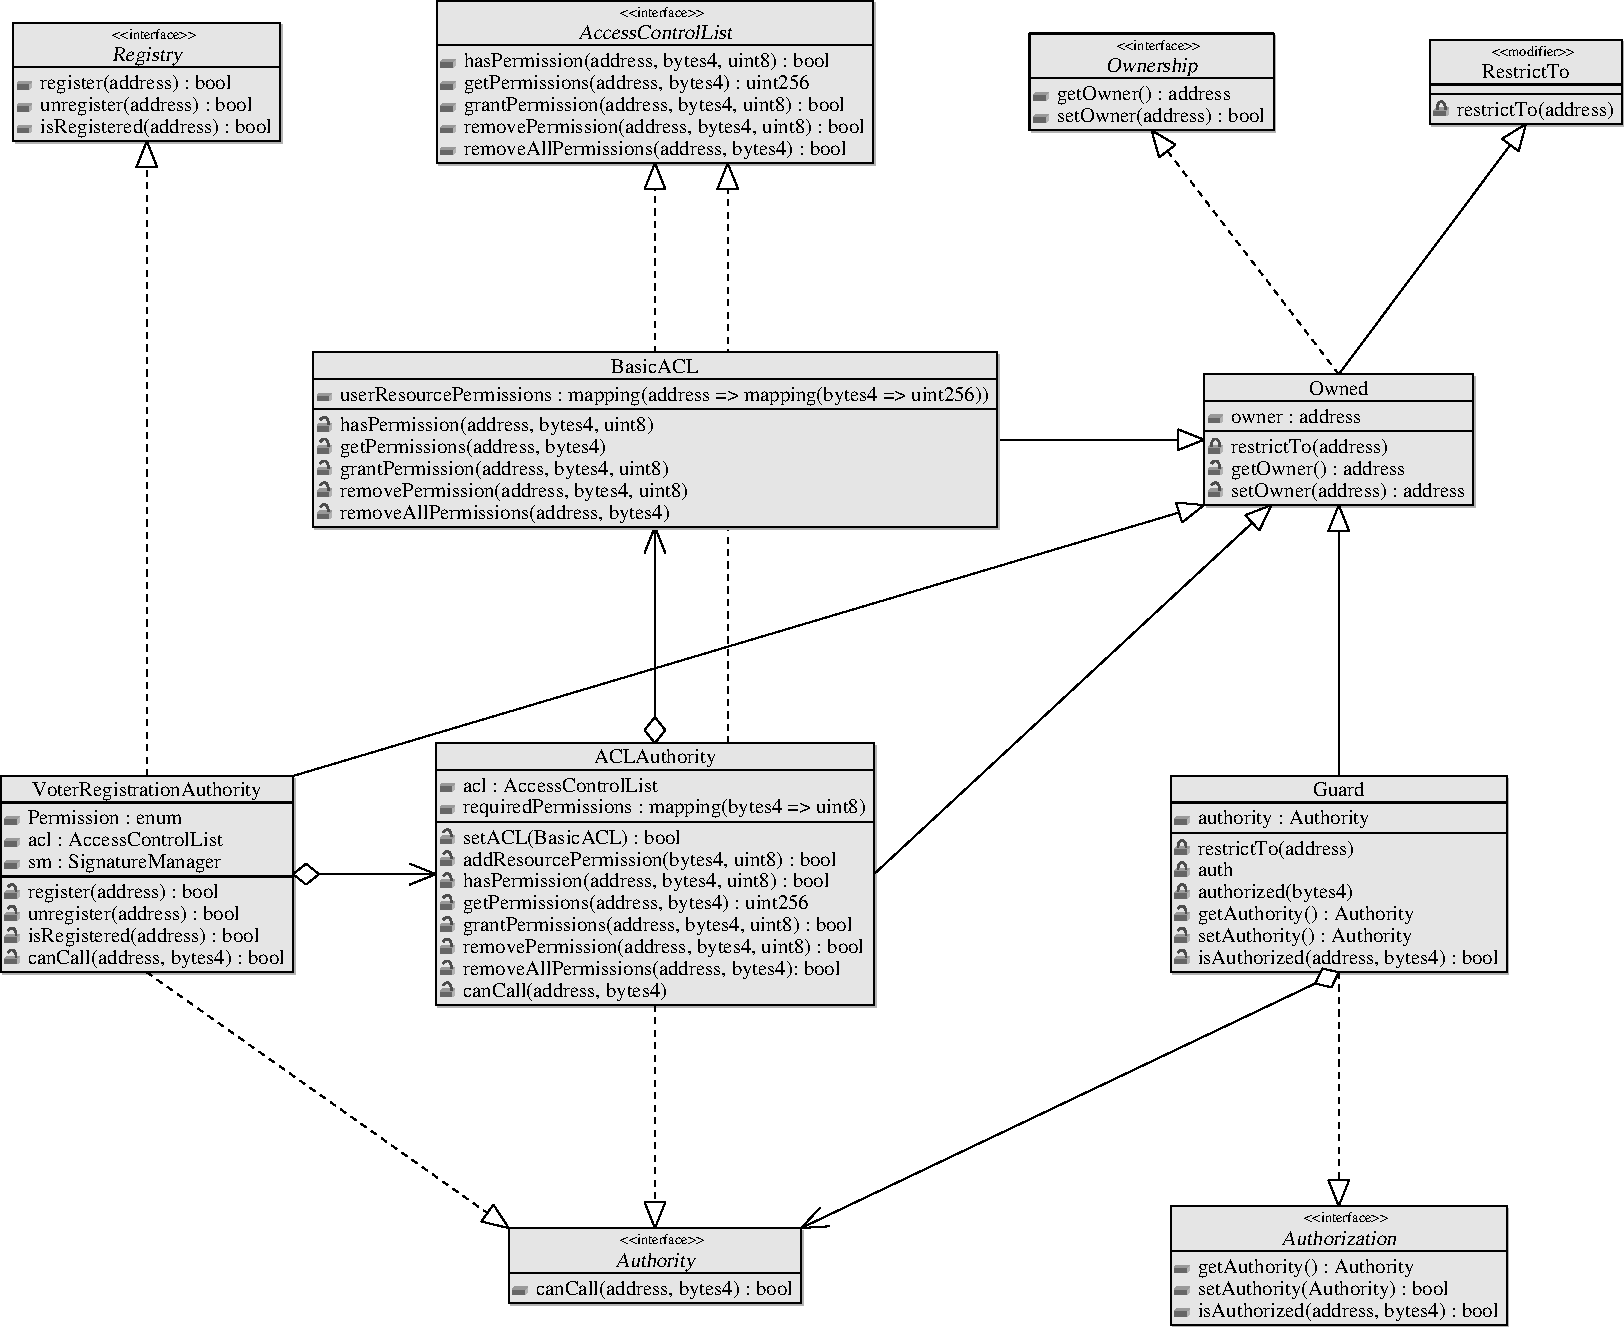
\includegraphics[width=\textwidth]{figures/authorization/figure}
  % \includestandalone[width=\textwidth]{\fig{authorization}}
\end{figure}

\subsubsection{Interface AccessControlList}

The \solt{interface}, \sol{interface AccessControlList}, introduces five
\solt{function} definitions to achieve basic access control list functionality:

\begin{enumerate}
  \item \sol{function hasPermission}, which validates that a \emph{subject} has
    the \emph{permission} required access some \emph{resource}.

  \item \sol{function getPermissions}, which returns the \emph{permissions} some
    \emph{subject} has for a given \emph{resource}.

  \item \sol{function setPermissions}, which updates the \emph{permissions} some
    \emph{subject} has for a given \emph{resource}.

  \item \sol{function grantPermission}, which grants a single \emph{permission}
    for some \emph{subject} with respect to some \emph{resource}.

  \item \sol{function revokePermission}, which revokes a single
    \emph{permission} for some \emph{subject} with respect to some
    \emph{resource}.
\end{enumerate}

\begin{solidity}[interface AccessControlList]
interface AccessControlList {
  function hasPermission (address _subject, bytes4 _resource, uint8 _permission)
    public view returns (bool _hasPermission);

  function getPermissions (address _subject, bytes4 _resource)
    public view returns (uint256 _permissions);

  function setPermissions (address _subject, bytes4 _resource, uint256 _permissions)
    public returns (bool _success);

  function grantPermission (address _subject, bytes4 _resource, uint8 _permission)
    public returns (bool _success);

  function revokePermission (address _subject, bytes4 _resource, uint8 _permission)
    public returns (bool _success);
}
\end{solidity}

\begin{interface}
  \begin{functions}
    \item \sol{function hasPermission (address _subject, bytes4 _resource, uint8 _permission)},
      evaluates whether some \emph{subject} has the requisite \emph{permission}
      to access some \emph{resource}.
      \begin{parameters}
        \item \sol{address _subject}, the \solt{address} of an account
          representing the \emph{subject}, i.e., the \emph{user}, to evaluate
          permissions against.
        \item \sol{bytes4 _resource}, the \emph{resource}, signature hash of a
          Solidity \solt{function}, to validate \emph{permissions} against.
        \item \sol{uint8 _permission}, a \emph{permission} level, or
          \emph{action}, which is being validated.
      \end{parameters}
      \begin{returns}
        \item \sol{bool _hasPermission}, returns the \solt{true} if the
            \emph{subject} has the requisite \emph{permission} to access the
            \emph{resource}, otherwise \solt{false}.
      \end{returns}

    \item \sol{function getPermissions (address _subject, bytes4 _resource)},
      retrieves the \emph{permissions}, for a \emph{<subject, resource>} pair.

      \begin{parameters}
        \item \sol{address _subject}, the account \solt{address} of the
          \emph{subject} whose \emph{permissions} are to be retrieved.

        \item \sol{bytes4 _resource}, the \emph{resource}, \solt{function}
          signature, which the \emph{permissions} should be retrieved for.
      \end{parameters}

      \begin{returns}
      \item \sol{uint256 _permissions}, the \solt{uint256} representation of the
        \emph{subject's} \emph{permissions} for a given \emph{resource}.
      \end{returns}

    \item \sol{function setPermissions (address _subject, bytes4 _resource, uint256 _permissions)},
      updates a \emph{subject's} \emph{permissions} for some \emph{resource}.

      \begin{parameters}
        \item \sol{address _subject}, the account \solt{address} of the
          \emph{subject} whose \emph{permissions} are to be modified.

        \item \sol{bytes4 _resource}, the \emph{resource}, \solt{function}
          signature, which the \emph{permissions} are to be modified for.

        \item \sol{uint256 _permissions}, the \solt{uint256} representation of
          the \emph{subject's} new \emph{permissions} for the \emph{resource}.
      \end{parameters}

      \begin{returns}
      \item \sol{bool _success}, resolves to \solt{true} if the operation was
        successful, otherwise \solt{false}.
      \end{returns}

    \item \sol{function grantPermission (address _subject, bytes4 _resource, uint8 _permission)},
      grants a \emph{subject} some \emph{permission} for a given \emph{resource}.

      \begin{parameters}
        \item \sol{address _subject}, the account \solt{address} of the
          \emph{subject} whose \emph{permissions} are to be modified.

        \item \sol{bytes4 _resource}, the \emph{resource}, \solt{function}
          signature, which the \emph{permissions} are to be modified for.

        \item \sol{uint8 _permission}, a \solt{uint8} value representing the
          \emph{permission-bit} to enable for the \emph{<subject, resource>}
          pair.
      \end{parameters}

      \begin{returns}
      \item \sol{bool _success}, resolves to \solt{true} if the operation was
        successful, otherwise \solt{false}.
      \end{returns}

    \item \sol{function revokePermission (address _subject, bytes4 _resource, uint8 _permission)},
      revokes a \emph{subject's} \emph{permission} for a given \emph{resource}.

      \begin{parameters}
        \item \sol{address _subject}, the account \solt{address} of the
          \emph{subject} whose \emph{permissions} are to be modified.

        \item \sol{bytes4 _resource}, the \emph{resource}, \solt{function}
          signature, which the \emph{permissions} are to be modified for.

        \item \sol{uint8 _permission}, a \solt{uint8} value representing the
          \emph{permission-bit} to revoke for the \emph{<subject, resource>}
          pair.
      \end{parameters}
      \begin{returns}
        \item \sol{bool _success}, resolves to \solt{true} if the operation was
          successful, otherwise \solt{false}.
      \end{returns}
  \end{functions}
\end{interface}

% \paragraph{function hasPermission}
%
% \subparagraph{Parameters}
% \begin{enumerate}
%   \item \sol{address _subject}, which represents some \emph{subject}, or
%         \emph{user}, accessing some \emph{resource}.
%   \item \sol{bytes4 _resource}, a \emph{resource}, or Solidity
%         \solt{function}, to validate \emph{permissions} against.
%   \item \sol{uint8 _permission}, a \emph{permission} level, or \emph{action},
%         which is being validated.
% \end{enumerate}
%
% \subparagraph{Returns}
% \sol{function hasPermission} is expected to \solt{return} a \solt{bool},
% \sol{bool _hasPermission}, which resolves to \solt{true} if the
% \emph{subject} has permission to access the \emph{resource}, Solidity
% \solt{function} associated with \sol{bytes4 _resource}, at the
% \emph{permission} level specified by \sol{uint8 _permission}.
%
% \paragraph{function getPermissions}
% \subparagraph{Parameters}
% \subparagraph{Returns}
%
% \paragraph{function setPermissions}
% \subparagraph{Parameters}
% \subparagraph{Returns}
%
% \paragraph{function grantPermission}
% \subparagraph{Parameters}
% \subparagraph{Returns}
%
% \paragraph{function removePermission}
% \subparagraph{Parameters}
% \subparagraph{Returns}
%


\subsubsection{Contract BasicACL}

The \solt{contract}, \sol{contract BasicACL}, implements the ACL
\solt{interface}, \sol{interface AccessControlList}, to provide a primitive
ACL implementation. The \solt{contract} implementation is backed by a mapping of
references, from \emph{subject} to \emph{resource} to \emph{permissions} --- as
described in Chapter~\ref{chap:methods}, \emph{\nameref{chap:methods}} --- i.e.,
a nested sparse vector mapping.

\begin{solidity}[contract BasicACL]
contract BasicACL is Owned, AccessControlList {
  mapping (address => mapping (bytes4 => uint256)) subjectResourcePermissions;

  function hasPermission (address _subject, bytes4 _resource, uint8 _permission) public constant restrictTo(owner) returns (bool _hasPermission) {
    uint256 result = subjectResourcePermissions[_subject][_resource] & (uint256(1) << _permission);
    return (result > 0);
  }

  function getPermissions (address _subject, bytes4 _resource) public constant restrictTo(owner) returns (uint256 _permissions) {
    return subjectResourcePermissions[_subject][_resource];
  }

  function grantPermission (address _subject, bytes4 _resource, uint8 _permission) public restrictTo(owner) returns (bool _success) {
    subjectResourcePermissions[_subject][_resource] |= uint256(1) << _permission;
    return true;
  }

  function revokePermission (address _subject, bytes4 _resource, uint8 _permission) public restrictTo(owner) returns (bool _success) {
    subjectResourcePermissions[_subject][_resource] &= ~(uint256(1) << _permission);
    return true;
  }

  function setPermissions (address _subject, bytes4 _resource, _permissions) public restrictTo(owner) returns (bool _success) {
    subjectResourcePermissions[_subject][_resource] = _permissions;
    return true;
  }
}
\end{solidity}

\begin{state}
  \begin{public}
    \item \sol{mapping (address => mapping (bytes4 => uint256)) subjectResourcePermissions}
      a nesting mapping used to record the \emph{permissions} which
      \emph{subjects} have to access various \emph{resources}.

      \begin{displayquote}
        Here \emph{subjects} are represented and identified by their account
        \solt{address}; \emph{resources} are assumed to be \solt{function}
        signatures, \solt{bytes4}; and \emph{permissions} are bit vectors,
        backed by \solt{uint256} values, where bit masks are leveraged to
        retrieve individual \emph{permission} values.
      \end{displayquote}
  \end{public}
\end{state}

\begin{code}
  \begin{functions}
    \item \sol{function hasPermission (address _subject, bytes4 _resource, uint8 _permission)},
      evaluates whether some \emph{subject} has the requisite \emph{permission}
      to access some \emph{resource}.

      \begin{displayquote}
        \emph{Permission} evaluation occurs by:
        \begin{enumerate}
          \item retrieving the \emph{permissions} bit vector from the
            \solt{mapping} \sol{subjectResourcePermissions}, where the
            \emph{subject}, \sol{address _subject}, and \emph{resource},
            \sol{bytes4 _resource}, are used as keys;

          \item creating a \emph{permission} bit mask by left-shifting 1
            \sol{_permission} times, \sol{1 << _permission};

          \item evaluating \sol{permissions |$\land$| bit_mask}; and finally,

          \item returning \solt{true} if the value resulting from the evaluation
            is greater than 0, i.e., the \emph{subject} has \emph{permission} to
            access to the \emph{resource}.
        \end{enumerate}
      \end{displayquote}

      \begin{parameters}
        \item \sol{address _subject}, the \solt{address} of an account
          representing the \emph{subject}, i.e., the \emph{user}, to evaluate
          permissions against.
        \item \sol{bytes4 _resource}, the \emph{resource}, signature hash of a
          Solidity \solt{function}, to validate \emph{permissions} against.
        \item \sol{uint8 _permission}, a \emph{permission} level, or
          \emph{action}, which is being validated.
      \end{parameters}

      \begin{returns}
        \item \sol{bool _hasPermission}, returns the \solt{true} if the
          \emph{subject} has the requisite \emph{permission} to access the
          \emph{resource}, otherwise \solt{false}.
      \end{returns}

    \item \sol{function getPermissions (address _subject, bytes4 _resource)},
      retrieves the \emph{permissions}, for a \emph{<subject, resource>} pair.

      \begin{parameters}
        \item \sol{address _subject}, the account \solt{address} of the
          \emph{subject} whose \emph{permissions} are to be retrieved.

        \item \sol{bytes4 _resource}, the \emph{resource}, \solt{function}
          signature, which the \emph{permissions} should be retrieved for.
      \end{parameters}

      \begin{returns}
      \item \sol{uint256 _permissions}, the \solt{uint256} representation of the
        \emph{subject's} \emph{permissions} for a given \emph{resource}.
      \end{returns}

    \item \sol{function setPermissions (address _subject, bytes4 _resource, uint256 _permissions)},
      updates a \emph{subject's} \emph{permissions} for some \emph{resource}.

      \begin{modifiers}
        \item \sol{modifier restrictTo (owner)}, restricts access to the
          \solt{function} such that \emph{only} the current \solt{owner} of the
          \solt{contract} can call it.
      \end{modifiers}

      \begin{parameters}
        \item \sol{address _subject}, the account \solt{address} of the
          \emph{subject} whose \emph{permissions} are to be modified.

        \item \sol{bytes4 _resource}, the \emph{resource}, \solt{function}
          signature, which the \emph{permissions} are to be modified for.

        \item \sol{uint256 _permissions}, the \solt{uint256} representation of
          the \emph{subject's} new \emph{permissions} for the \emph{resource}.
      \end{parameters}

      \begin{returns}
        \item \sol{bool _success}, resolves to \solt{true} if the operation was
          successful, otherwise \solt{false}.
      \end{returns}

    \item \sol{function grantPermission (address _subject, bytes4 _resource, uint8 _permission)},
      grants a \emph{subject} \emph{permission} for a given \emph{resource}.

      \begin{displayquote}
        \emph{Permission} grant occurs by:
        \begin{enumerate}
          \item retrieving the \emph{permissions} bit vector from the
            \solt{mapping} \sol{subjectResourcePermissions}, where the
            \emph{subject}, \sol{address _subject}, and \emph{resource},
            \sol{bytes4 _resource}, are used as keys;

          \item creating a \emph{permission} bit mask by left-shifting 1
            \sol{_permission} times, \sol{1 << _permission};

          \item evaluating \sol{permissions |$\lor$| bit_mask} to produce a new
            \emph{permissions} bit vector; and finally,

          \item updating the state of the \solt{contract} by storing the
            resulting \emph{permissions} bit vector back into the
            \sol{subjectResourcePermissions} \solt{mapping}.
        \end{enumerate}
      \end{displayquote}

      \begin{modifiers}
        \item \sol{modifier restrictTo (owner)}, restricts access to the
          \solt{function} such that \emph{only} the current \solt{owner} of the
          \solt{contract} can call it.
      \end{modifiers}

      \begin{parameters}
        \item \sol{address _subject}, the account \solt{address} of the
          \emph{subject} whose \emph{permissions} are to be modified.

        \item \sol{bytes4 _resource}, the \emph{resource}, \solt{function}
          signature, which the \emph{permissions} are to be modified for.

        \item \sol{uint8 _permission}, a \solt{uint8} value representing the
          \emph{permission-bit} to enable for the \emph{<subject, resource>}
          pair.
      \end{parameters}

      \begin{returns}
      \item \sol{bool _success}, resolves to \solt{true} if the operation was
        successful, otherwise \solt{false}.
      \end{returns}

    \item \sol{function revokePermission (address _subject, bytes4 _resource, uint8 _permission)},
      revokes a \emph{subject's} \emph{permission} for a given \emph{resource}.

      \begin{displayquote}
        \emph{Permission} revocation occurs by:
        \begin{enumerate}
          \item retrieving the \emph{permissions} bit vector from the
            \solt{mapping} \sol{subjectResourcePermissions}, where the
            \emph{subject}, \sol{address _subject}, and \emph{resource},
            \sol{bytes4 _resource}, are used as keys;

          \item creating a \emph{permission} bit mask by left-shifting 1
            \sol{_permission} times, \sol{1 << _permission};

          \item flipping all of the bits of the \emph{permission} bit mask,
            \sol{~bit_mask};

          \item evaluating \sol{permissions |$\land$| bit_mask} to produce a new
            \emph{permissions} bit vector; and finally,

          \item updating the state of the \solt{contract} by storing the
            resulting \emph{permissions} bit vector back into the
            \sol{subjectResourcePermissions} \solt{mapping}.
        \end{enumerate}
      \end{displayquote}

      \begin{modifiers}
        \item \sol{modifier restrictTo (owner)}, restricts access to the
          \solt{function} such that \emph{only} the current \solt{owner} of the
          \solt{contract} can call it.
      \end{modifiers}

      \begin{parameters}
        \item \sol{address _subject}, the account \solt{address} of the
          \emph{subject} whose \emph{permissions} are to be modified.

        \item \sol{bytes4 _resource}, the \emph{resource}, \solt{function}
          signature, which the \emph{permissions} are to be modified for.

        \item \sol{uint8 _permission}, a \solt{uint8} value representing the
          \emph{permission-bit} to revoke for the \emph{<subject, resource>}
          pair.
      \end{parameters}

      \begin{returns}
      \item \sol{bool _success}, resolves to \solt{true} if the operation was
        successful, otherwise \solt{false}.
      \end{returns}
  \end{functions}
\end{code}


\subsubsection{Contract ACLAuthority}

The \solt{contract}, \sol{contract ACLAuthority}, merges the ACL functionality
introduced by \sol{interface AccessControlList} with the generalized access
control functionality introduced by \sol{interface Authority}.

\begin{solidity}[contract ACLAuthority]
contract ACLAuthority is Owned, Authority, AccessControlList {
  AccessControlList acl;
  mapping (bytes4 => uint8) requiredResourcePermission;

  constructor (bool _createACL) {
    if (_createACL) acl = new BasicACL();
  }

  function hasPermission (address _subject, bytes4 _resource, uint8 _permission) public constant returns (bool _hasPermission) {
    return acl.hasPermission(_subject, _resource, _permission);
  }

  function getPermissions (address _subject, bytes4 _resource) public constant returns (uint256 _permissions) {
    return acl.getPermissions(_subject, _resource);
  }

  function grantPermission (address _subject, bytes4 _resource, uint8 _permission) public restrictTo(owner) returns (bool _success) {
    return acl.grantPermission(_subject, _resource, _permission);
  }

  function revokePermission (address _subject, bytes4 _resource, uint8 _permission) public restrictTo(owner) returns (bool _success) {
    return acl.removePermission(_subject, _resource, _permission);
  }

  function setPermissions (address _subject, bytes4 _resource, uint256 _permissions) public restrictTo(owner) returns (bool _success) {
    return acl.setPermissions(_subject, _resource, _permissions);
  }

  function setACL(AccessControlList _acl) public restrictTo(owner) returns (bool _success) {
    assert(_acl.owner() == address(this));
    acl = _acl;
    return true;
  }

  function setRequiredResourcePermission (bytes4 _resource, uint8 _permission) public restrictTo(owner) returns (bool _success) {
    requiredResourcePermission[_resource] = _permission;
    return true;
  }

  function canCall (address _subject, bytes4 _resource) public constant returns (bool _canCall) {
    return hasPermission(_subject, _resource, requiredResourcePermission[_sig]);
  }
}
\end{solidity}

\begin{state}
  \begin{public}
  \item \sol{AccessControlList acl} maintains the \solt{address} of an ACL
    implementation, a \solt{contract} which implements \sol{interface
    AccessControlList}.

  \item \sol{mapping (bytes4 => uint8) requiredResourcePermissions} maintains a
    mapping of \solt{function}[s], \sol{bytes4}, to required
    \emph{permission}, \sol{uint8}.
  \end{public}
\end{state}

\begin{code}
  \begin{constructor}
  \item \sol{constructor (bool _createACL)}, upon creation and initialization
    of this \solt{contract} the \solt{constructor} can deploy a
    \solt{contract}, \sol{contract BasicACL}, if the \solt{bool}, \sol{bool
    _createACL}, is set to \solt{true}.

    \begin{parameters}
    \item \sol{bool _createACL}, set to \solt{true} to deploy an ACL
      implementation, \sol{contract BasicACL}, in addition to this
      \solt{contract}; otherwise \solt{false}.
    \end{parameters}
  \end{constructor}

  \begin{functions}
  \item \sol{function setAcl (AccessControlList _acl)}, updates the
    \solt{contract} reference which is responsible for managing ACL requests.

    \begin{modifiers}
    \item \sol{modifier restrictTo (owner)}, restricts access to the
      \solt{function} such that \emph{only} the current \solt{owner} of the
      \sol{contract} can call it.
    \end{modifiers}

    \begin{parameters}
    \item \sol{AccessControlList _acl}, the ACL implementation which access
      control responsibilities are to be delegated to.
    \end{parameters}

    \begin{returns}
    \item \sol{bool _success}, resolves to \solt{true} if the operation was
      successful, otherwise \solt{false}.
    \end{returns}


  \item \sol{function setRequiredResourcePermission (bytes4 _resource, uint8 _permission)},
    updates the mapping representing the \emph{permission} required to access
    some \emph{resource}, \solt{function} signature.

    \begin{modifiers}
    \item \sol{modifier restrictTo (owner)}, restricts access to the
      \solt{function} such that \emph{only} the current \solt{owner} of the
      \sol{contract} can call it.
    \end{modifiers}

    \begin{parameters}
    \item \sol{bytes4 _resource}, the \emph{resource}, \solt{function}
      signature, which the \emph{permission} is to be modified for.

    \item \sol{uint8 _permission}, a \solt{uint8} value representing the
      \emph{permission-bit} required for the \emph{resource}.
    \end{parameters}

    \begin{returns}
    \item \sol{bool _success}, resolves to \solt{true} if the operation was
      successful, otherwise \solt{false}.
    \end{returns}


  \item \sol{function canCall (address _subject, bytes4 _resource)}, evaluates
    whether a \emph{subject} can access to some \emph{resource} by validating
    with the ACL implementation that the \emph{subject} has the required
    \emph{resource} \emph{permission}.

    \begin{parameters}
    \item \sol{address _subject}, the \emph{subject}, Ethereum account,
      whose \emph{permissions} are being evaluated.

    \item \sol{bytes4 _resource}, the \emph{resource}, \solt{contract
      function}, which the \emph{subject's} \emph{permissions} are being
      evaluated against.
    \end{parameters}

    \begin{returns}
    \item \sol{bool _canCall}, resolves to \solt{true} if the
      \emph{subject}, \sol{address _subject}, is permitted to access the
      \emph{resource}, \sol{bytes4 _resource}, otherwise \solt{false}.
    \end{returns}


  \item
    \sol{function hasPermission (address _subject, bytes4 _resource, uint8 _permission)}, \\
    \sol{function getPermissions (address _subject, bytes4 _resource)}, \\
    \sol{function setPermissions (address _subject, bytes4 _resource, uint256 _permissions)}, \\
    \sol{function grantPermission (address _subject, bytes4 _resource, uint8 _permission)}, \\
    \sol{function revokePermission (address _subject, bytes4 _resource, uint8 _permission)}, \\
    all ACL responsibilities originating from \sol{interface AccessControlList}
    are delegated to the provided ACL implementation stored in
    \sol{AccessControlList acl}.

    \begin{modifiers}
    \item \sol{modifier restrictTo (owner)}, restricts access to the
      \solt{function} such that \emph{only} the current \solt{owner} of the
      \solt{contract} can call this \solt{function}; this applies to
      \solt{function}[s] \sol{setPermissions}, \sol{grantPermission}, and
      \sol{revokePermission}.
    \end{modifiers}
  \end{functions}
\end{code}



% Sub-section: Registries
\subsection{Registries}

Having completed the work of generalizing access control and building access
control lists, we now introduce a simplified access control model for managing
voter registration during elections.

\begin{enumerate}
  \item \sol{interface Registry}, which defines the functions for registering
    voters for an election, and
  \item \sol{contract VoterRegistrationAuthority}, which implements and
    aggregates several \solt{interface}[s] and \solt{interface} implementations
    --- namely \sol{interface Registry}, \sol{interface Authority}, and
    \sol{contract ACLAuthority} --- to build a trusted source of registered
    voters.
\end{enumerate}

\begin{figure}[H]
  \centering
  \figurepdf[]{registry}
  \caption{Simplified election registry.}\label{fig:registry}
  % 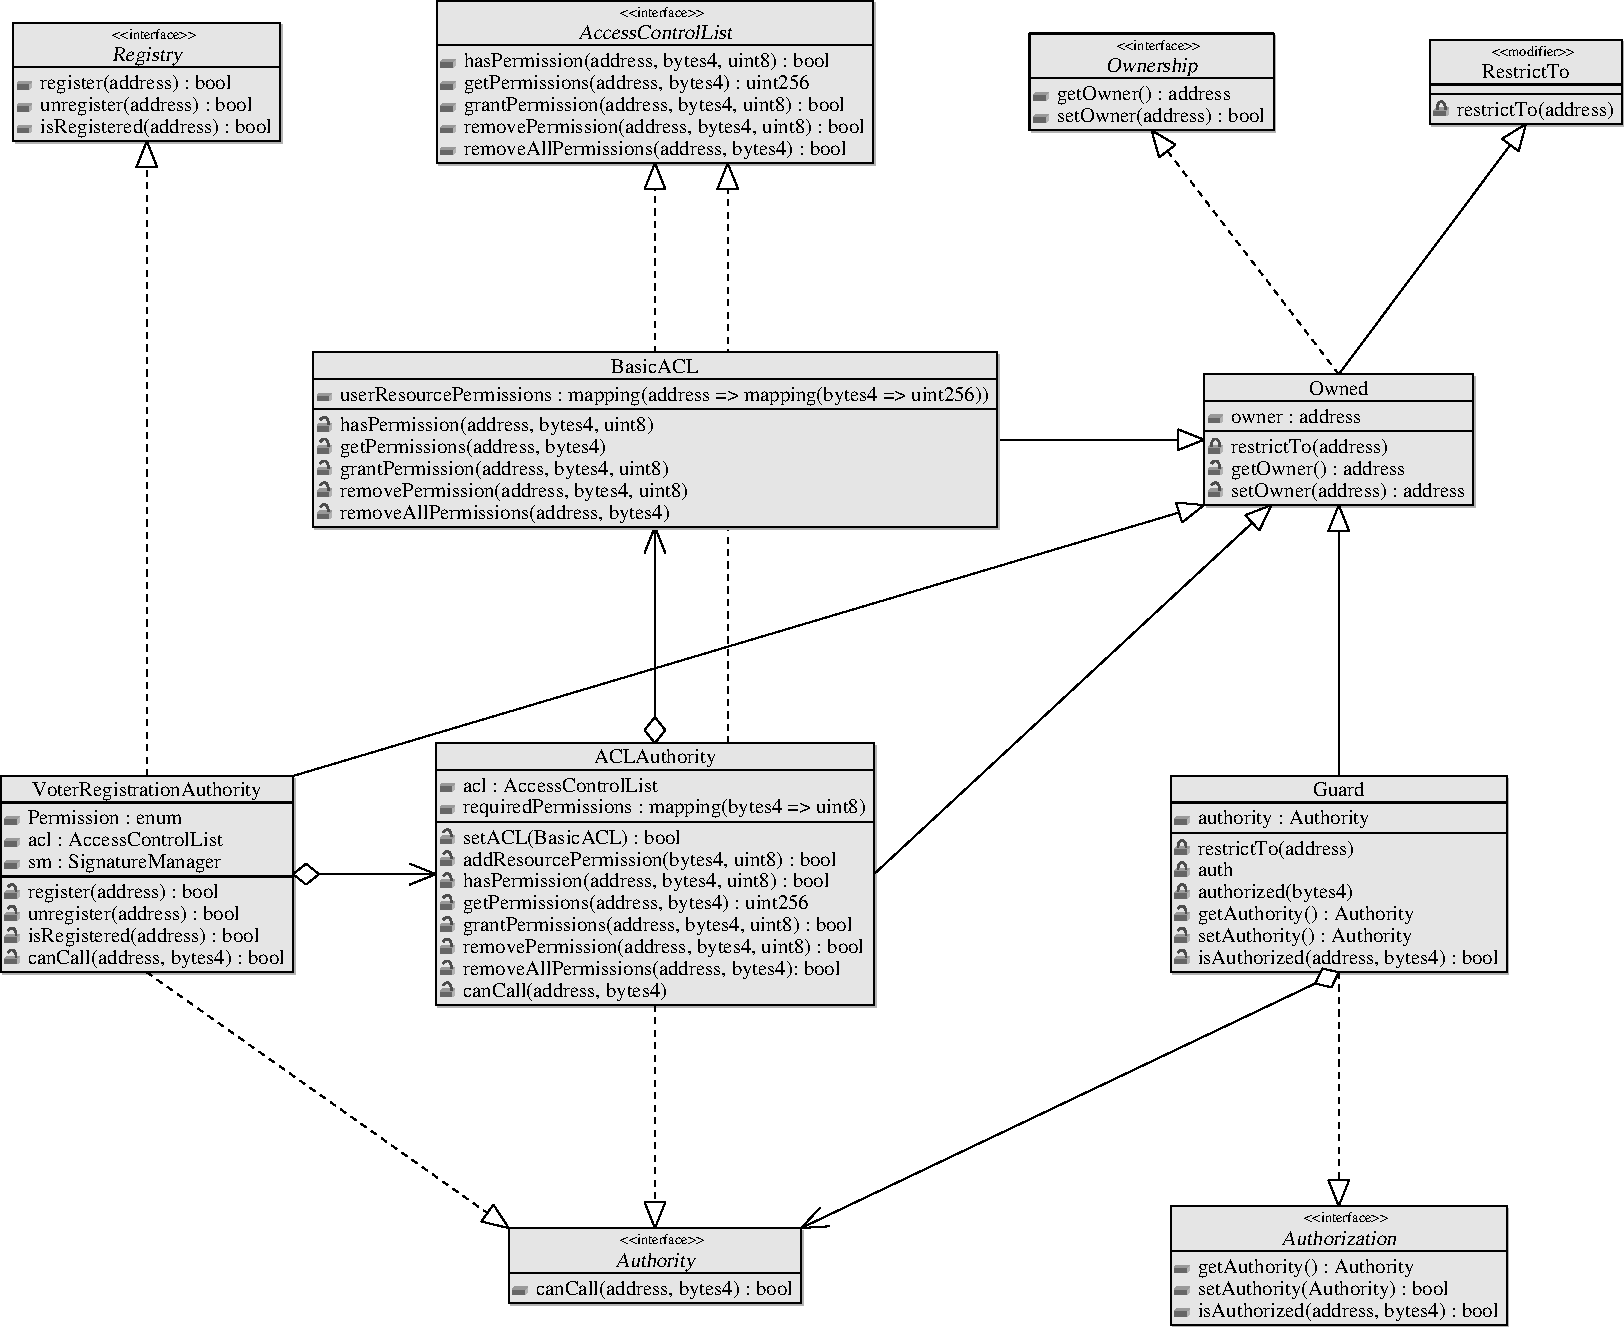
\includegraphics[width=\textwidth]{figures/authorization/figure}
  % \includestandalone[width=\textwidth]{\fig{authorization}}
\end{figure}

\subsubsection{Interface Registry}

The \solt{interface}, \sol{interface Registry}, introduces three \solt{function}
definitions required to achieve basic registry functionality:

\begin{enumerate}
  \item \sol{function register}, which \emph{registers} a \emph{subject}.

  \item \sol{function unregister}, which \emph{unregisters} a \emph{subject}.

  \item \sol{function isRegistered}, which evaluates whether a \emph{subject} is
    \emph{registered}.
\end{enumerate}

\begin{solidity}[interface Registry]
interface Registry {
  function register (address _subject) public returns (bool _success);
  function unregister (address _subject) public returns (bool _success);
  function isRegistered (address _subject) public constant returns (bool _isRegistered);
}
\end{solidity}

\begin{interface}
  \begin{functions}
    \item \sol{function isRegistered (address _subject)}, evaluates whether some
      \emph{subject} is \emph{registered}.

      \begin{parameters}
        \item \sol{address _subject}, the \solt{address} of an account
          representing the \emph{subject}, to evaluate the \emph{registration}
          of.
      \end{parameters}

      \begin{returns}
        \item \sol{bool _isRegistered}, returns the \solt{true} if the
          \emph{subject} is \emph{registered}, otherwise \solt{false}.
      \end{returns}

    \item \sol{function unregister (address _subject)}, \emph{unregisters} a
      \emph{subject}.

      \begin{parameters}
        \item \sol{address _subject}, the account \solt{address} of the
          \emph{subject} who is to be \emph{unregistered}.
      \end{parameters}

      \begin{returns}
        \item \sol{bool _success}, resolves to \solt{true} if the operation was
          successful, otherwise \solt{false}.
      \end{returns}

    \item \sol{function register (address _subject)}, \emph{registers} a
      \emph{subject}.

      \begin{parameters}
        \item \sol{address _subject}, the account \solt{address} of the
          \emph{subject} who is to be \emph{registered}.
      \end{parameters}

      \begin{returns}
        \item \sol{bool _success}, resolves to \solt{true} if the operation was
          successful, otherwise \solt{false}.
      \end{returns}
  \end{functions}
\end{interface}


\subsubsection{Contract VoterRegistrationAuthority}

The \solt{contract}, \sol{contract VoterRegistrationAuthority}, is the final
component of our authorization design and is required to construct a generalized
voter registration authority capable of managing registered voters and
conducting elections.

% signatureMap['vote'] = bytes4(sha3('vote(uint8[],uint8[])'));
\begin{solidity}[contract VoterRegistrationAuthority]
contract VoterRegistrationAuthority is Owned, Registry, Authority {
  enum Permissions {
    Vote
  }

  AccessControlList acl;
  mapping (bytes32 => bytes4) resourceSignatures;

  constructor () public {
    acl = new ACLAuthority(true);

    resourceSignatures['vote'] = bytes4(sha3('vote()'));

    acl.setRequiredResourcePermission(
      resourceSignature('vote'),
      uint8(Permissions.Vote)
    );
  }

  function register (address _voter) public restrictTo(owner) returns (bool _success) {
    return acl.grantPermission(_voter, resourceSignatures['vote'], uint8(Permissions.Vote));
  }

  function unregister (address _voter) public restrictTo(owner) returns (bool _success) {
    return acl.revokePermission(_voter, resourceSignatures['vote'], uint8(Permissions.Vote));
  }

  function isRegistered (address _voter) public constant returns (bool _isRegistered) {
    return acl.hasPermission(_voter, resourceSignatures['vote'], uint8(Permissions.Vote));
  }

  function canCall (address _subject, bytes4 _resource) public constant returns (bool _canCall) {
    return acl.canCall(_subject, _resource);
  }
}
\end{solidity}

\todo{Finish documenting the VoterRegistrationAuthority implementation.}

\begin{state}
  \begin{public}
    \item \sol{AccessControlList acl} maintains the \solt{address} of an ACL
      implementation, a \solt{contract} which implements \sol{interface
      AccessControlList}.

    \item \sol{mapping (bytes32 => bytes4) resourceSignatures} maintains a
      mapping of strings, \sol{bytes32}, to \solt{function} signature,
      \sol{bytes4}.
  \end{public}
\end{state}

\begin{code}
  \begin{constructor}
    \item \sol{constructor ()}, upon creation and initialization of this
      \solt{contract} the \solt{constructor} will deploy a \solt{contract},
      \sol{contract BasicACL}.
  \end{constructor}

  \begin{functions}
    \item \sol{function isRegistered (address _subject)}, evaluates whether some
      \emph{subject} is \emph{registered}.

      \begin{parameters}
        \item \sol{address _subject}, the \solt{address} of an account
          representing the \emph{subject}, to evaluate the \emph{registration}
          of.
      \end{parameters}

      \begin{returns}
        \item \sol{bool _isRegistered}, returns the \solt{true} if the
          \emph{subject} is \emph{registered}, otherwise \solt{false}.
      \end{returns}

    \item \sol{function unregister (address _subject)}, \emph{unregisters} a
      \emph{subject}.

      \begin{parameters}
        \item \sol{address _subject}, the account \solt{address} of the
          \emph{subject} who is to be \emph{unregistered}.
      \end{parameters}

      \begin{returns}
        \item \sol{bool _success}, resolves to \solt{true} if the operation was
          successful, otherwise \solt{false}.
      \end{returns}

    \item \sol{function register (address _subject)}, \emph{registers} a
      \emph{subject}.

      \begin{parameters}
        \item \sol{address _subject}, the account \solt{address} of the
          \emph{subject} who is to be \emph{registered}.
      \end{parameters}

      \begin{returns}
        \item \sol{bool _success}, resolves to \solt{true} if the operation was
          successful, otherwise \solt{false}.
      \end{returns}
  \end{functions}
\end{code}


